\section{Developed scripts}
\label{s:Scripts}
For the purpose of automating the issuing of tasks to each worker, automatic collection of packet captures, and retrieval of all packet captures from each worker, code had to be produced to achieve this goal. The scripts developed in this research are further described in each respective subsection in this section.



\subsection{Scanner}
\label{s:ScannerScript}
Given task files are iterated until a task with the status new is found.
From this point, the scanner host deploys a task to the worker through the management network, commanding it to dump traffic on the incoming interface pointed to the scanning network.
When this task is successfully deployed, the scanner hosts start the scan on the scanning network towards the worker with the given scanning characteristics. As a default in this script, using the Nmap scanner, the result of the scan from the scanner host is outputted to an XML result file represented with the given task name. This XML file is not used for analysis within this research, though the generated XML file could be used in future work, further described in section \ref{s:ConclusionFutureWork}. The status for the representative task in the task file is changed from $new$ to $ongoing$. This operation is iterated through all workers until all workers are busy when the scanning host cannot deploy more tasks until one or more of the workers are available for work again. A capture of this is shown in figure \ref{fig:LabTaskAllocation}.

The scanner script is built up with a number of functions for later use within the script.

\subsubsection{Standardising the message output}
When the script is running from the prompt by a user, it is important that the output is human-readable.
The function in listing å\ref{lst:ColorizeMsg} colorizes the messages depending on error messages, success messages, or ordinary messages.
A visualization of this output is shown in figure \ref{fig:LabTaskAllocation}. The figure also shows the message output when conducting task allocation, further elaborated in section \ref{ss:DeployingTasks}.

\begin{listing}[!ht]
\caption{Colorizing messages}
\label{lst:ColorizeMsg}
\begin{minted}{Bash}
colored_message() {
  COLOR=$1
  MESSAGE="$2"
  if [[ $COLOR == "red" ]]; then
    echo -e "[ \e[31m\e[1mError\e[0m ] $MESSAGE"
  elif [[ $COLOR == "green" ]]; then
    echo -e "[ \e[32m\e[1mSuccess\e[0m ] $MESSAGE"
  else
    echo -e "$MESSAGE"
  fi
}
\end{minted}
\end{listing}

\begin{figure}[htbp]
\centerline{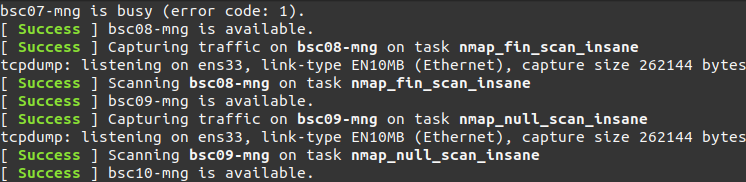
\includegraphics[scale=0.6]{images/lab/taskissuing.png}}
\caption{Capture of task allocation and a standardized colorized message format.}
\label{fig:LabTaskAllocation}
\end{figure}





\subsubsection{Checking task status}
\label{ss:CheckTaskStatus}
The input for this function is the unique task name.
The function would then retrieve the process information for the given task name.
It will then check if the indicated process ID on the scanner machine exists, and the result would be returned in the format where \textit{1} symbolize that the task is still in progress, while \textit{0} would identify a task complete.

\begin{listing}[!ht]
\caption{Checking scan status}
\label{lst:CheckScanStatus}
\begin{minted}{Bash}
check_scan_status() {
  TASK_NAME=$1
  SCANNER_PROCESS_INFO=$(ps aux | grep "${RESULT_DIR}/${TASK_NAME}" | grep -v grep)
  SCANNER_LOCAL_PID=$(echo $SCANNER_PROCESS_INFO | awk '{ print $2 }')

  if [[ ! -z $SCANNER_LOCAL_PID ]]; then
    return 1 # return false - still working
  else
    return 0 # return true - work done
  fi
}
\end{minted}
\end{listing}

As seen in listing \ref{lst:CheckScanStatus} the if statement checks if a process ID is set with the statement that the process ID should not (using $!$) be a zero value ($z$).
If the process ID is not set, it will return an error code $1$ ($false$ in this case), while the error code $0$ ($true$ in this case) is returned if the process ID is zero.
This goes against the general logic in programming, where usually $1$ is $true$ and $0$ is $false$.
The reason for returning $1$ in Bash is that it returns the error code given from the script. A $0$ error code indicates no errors and will therefore be true, while any other positive error codes would indicate an error.
This could be not only applied for the Bash shell but also in system error codes used in Windows, where $0$ ($0x0$) is a successful operation \autocite{MicrosoftErrorCode}.

\subsubsection{Terminate a given task}
\label{ss:TerminateTask}
The input for this function is the unique task name.
The function would retrieve the process information for the given task name.
If the given process ID is found, the script will continue to retrieve the local PID on the scanner host and retrieve the remote process information running on the respective worker host.
The local process on the scanner host would be killed, and the remote process ID's allocated to the tcpdump running with the unique task name would be gracefully killed as well.

\begin{listing}[!ht]
\caption{Terminate tcpdump}
\label{lst:TerminateTcpDump}
\begin{minted}{Bash}
terminate_tcpdump() {
  TASK_NAME=$1
  PROCESS_INFO=$(ps aux | grep -E "(tcpdump).*($TASK_NAME)" | grep -v grep)
  if [[ ! -z $PROCESS_INFO ]]; then
    LOCAL_PID=$(echo $PROCESS_INFO | awk '{ print $2 }')
    WORKER_HOST=$(echo $PROCESS_INFO | awk -F 'ssh' '{ print $2 }' | \
    awk '{ print $1 }')
    REMOTE_PIDS=$(ssh $WORKER_HOST ps aux | grep -E "(tcpdump).*($TASK_NAME)" | \
    awk '{ print $2 }')
    REMOTE_PIDS_VIEW=$(echo $REMOTE_PIDS | tr "\n" " ")

    kill -15 $LOCAL_PID ; ssh $WORKER_HOST kill -15 $REMOTE_PIDS_VIEW
    STATUS=$?
    return $STATUS
  fi
}
\end{minted}
\end{listing}

After the process is gracefully killed, the function would return the status of the executed command for use where the function is executed in the script.

\subsubsection{Availability check}
\label{ss:AvailabilityCheck}
The primary mission of this function is to determine if a worker is busy or available for work.
The input for this function is the given hostname, which will be collated to the tcpdump process on the respective worker.
There exist multiple status checks for the worker.
Mainly the function returns three various types of status; unreachable, busy, or available.
Since the scanner is attempting to SSH into the given worker host, and no reply is given, an unreachable status is returned from the function. If SSH is successful and a process with tcpdump is running on the given worker, the busy status is returned. If none of these checks are true, the status available would be returned.

\begin{listing}[!ht]
\caption{Retrieving available workers}
\label{lst:AvailableWorker}
\begin{minted}{Bash}
available_worker() {
  HOSTNAME=$1
  PID_TCPDUMP=$(ssh -q $HOSTNAME pgrep tcpdump)
  if ! ssh -q -T $HOSTNAME exit &> /dev/null; then
    return 2 # unreachable
  elif [[ ! -z $PID_TCPDUMP ]]; then
    return 1 # busy
  else
    return 0 # available
  fi
}
\end{minted}
\end{listing}


\subsubsection{Task status change}
\label{ss:TaskStatusChange}
Since the scanner script iterates through the task list, a function for changing the given task status was crucial to integrate for task management.
There exist four different inputs to this function; unique task name, priority, old status, and new status.
This function would generate an old and new CSV formatted entry.
This format is later used to replace the given old string in the CSV task file with the new string.
When successfully completed, a success return is given, while an error return is given if the command fails.

\begin{listing}[!ht]
\caption{Changing task status}
\label{lst:TaskChange}
\begin{minted}{Bash}
task_change() {
  TASK_NAME=$1
  PRIORITY=$2
  OLD_STATUS=$3
  NEW_STATUS=$4

  OLD_CSV_ENTRY="$PRIORITY,$TASK_NAME,$OLD_STATUS"
  NEW_CSV_ENTRY="$PRIORITY,$TASK_NAME,$NEW_STATUS"

  if sed -i -e "s/$OLD_CSV_ENTRY/$NEW_CSV_ENTRY/g" $TASK_FILE; then
    return 0 # true (success)
  else
    return 1 # false (error)
  fi
}
\end{minted}
\end{listing}

\subsubsection{Find interface name and start tcpdump}
The need to know which interface tcpdump should listen to is solved through a function.
Input to this function is the given worker hostname.
The function logs into the worker and extracts the interface name from the given subnet.

\begin{listing}[!ht]
\caption{Find scanning network interface on worker host}
\label{lst:ScanNIC}
\begin{minted}{Bash}
find_listening_scanner_if() {
  WORKER_HOST=$1
  IF=$(ssh $WORKER_HOST ip r | grep $SUBNET | awk '{print $3}')
  echo $IF
}
\end{minted}
\end{listing}

With the knowledge of the network interface name on the worker, tcpdump could be started.
Into this function are the worker's hostname and the output packet capture filename.
This function starts the tcpdump on the given worker through SSH with the output to the given packet capture file.
It returns then the status for the task, where `1` is returned as successfully started or `0` if the command failed to execute.
Within the start of the script, a filter parameter is given as a default filter for all the conducted scans, denoted in the first line below.

\begin{minted}{Bash}
TCPDUMP_FILTER="ip and dst not 192.168.2.1 and src not 192.168.2.1" # no GW tfc

start_tcpdump() {
  WORKER_HOST=$1
  PCAP_FILENAME=$2
  INTERFACE=$(find_listening_scanner_if $WORKER_HOST)

  if ssh $WORKER_HOST "tcpdump -U -i $INTERFACE -w $PCAP_FILENAME $TCPDUMP_FILTER \
  2>&1" & > /dev/null; then
    return 0 # success!
  else
    return 1
  fi
}
\end{minted}

\subsubsection{Scanner function}
\label{ss:ScannerFunction}
The scan itself is conducted within this function.
Inputs to this function are which scanner is to be used (e.g., Nmap), the worker's hostname, the output path for the XML generated from the scanner, and additional arguments used for the scan.
The function starts the scanner and returns an error code to symbolize successfully started or failed to start.

\begin{listing}[!ht]
\caption{Scanning function}
\label{lst:Scan}
\begin{minted}{Bash}
scan() {
  SCANNER=$1
  TARGET_HOST=$2
  OUTPUT_PATH=$3
  SCANNER_ARGS="$4" # must do something like ${4.<endline>}
  SCANNER_ARGS=$(echo $SCANNER_ARGS | sed 's/"//g')

  # Nmap
  if [ $SCANNER == "nmap" ]; then
    nmap -oX $OUTPUT_PATH.xml $TARGET_HOST $SCANNER_ARGS --system-dns 2>&1 \
    > /dev/null &
    ERR_CODE=$?
    return $ERR_CODE
  fi
}
\end{minted}
\end{listing}

\subsubsection{Task list update}
\label{ss:TaskListUpdate}
This function iterates through the task list, reading the values for each task from a CSV task file.
It checks if a valid task name is given and detects if a header is found.
The status for the given task name is checked through the task status check function \ref{ss:CheckTaskStatus}.
If the status `0` is returned, which symbolizes work done, this function would terminate tcpdump, as seen in listing  \ref{lst:TerminateTcpDump}.

\begin{listing}[!ht]
\caption{Update tasklist and terminate TCPDump when scan is complete}
\label{lst:UpdateTasklist}
\begin{minted}{Bash}
update_tasklist() {
  # Read through the tasks in the task file
  while IFS=, read -r PRIORITY TASK_NAME TASK_STATUS SCANNER EXTRA_ARGS
  do
    # Make sure that the task is not the header in the task file
    if [[ ! -z $TASK_NAME ]] && [[ $TASK_NAME != "task_name" ]]; then
      check_scan_status $TASK_NAME
      SCAN_STATUS=$?

      if [[ $SCAN_STATUS -eq 0 ]]; then
        if terminate_tcpdump $TASK_NAME; then
          task_change $TASK_NAME $PRIORITY "ongoing" "completed"
        else
          colored_message "red" \
          "Unable to terminate traffic capture on task \e[1m${TASK_NAME}\e[0m."
        fi
      fi
    fi
  done < $TASK_FILE
}
\end{minted}
\end{listing}

\subsubsection{Deploying tasks to a worker}
\label{ss:DeployingTasks}
Within this function of the scanner script, the deployment of tasks is conducted to a given worker.
This function requires the input of a given worker host.
Furthermore, it iterates through the task list and determines which tasks have the status new.
Tcpdump is then attempted to be started on the given worker.
When tcpdump is successfully started on the worker, it starts the scanning towards the given worker.
The status in the task list is changed from new to ongoing.
If the steps of either starting tcpdump or scan fail, an error message is given.
When a task is deployed successfully, the iteration will break and stop.

\begin{listing}[!ht]
\caption{Deploy tasks to a worker host}
\label{lst:DeployTaskWorker}
\begin{minted}{Bash}
deploy_tasks_to_worker() {

  # Define worker host
  WORKER_HOST=$1

  # Read through the tasks in the task file
#    update_tasklist

  while IFS=, read -r PRIORITY TASK_NAME TASK_STATUS SCANNER EXTRA_ARGS
  do
    # Make sure that the task is not the header in the task file
    if [[ ! -z $TASK_NAME ]] && [[ $TASK_NAME != "task_name" ]]; then

      # Do not scan the management side
      TARGET_HOST=$(echo $WORKER_HOST | sed 's/-mng//g')
      # -------------------
      # Task status: NEW - deploy tasks to worker
      # -------------------
      if [[ $TASK_STATUS == "new" ]]; then
        TIMESTAMP=$(date +%Y%m%d%H%M)
        OUTPUT_PATH="${RESULT_DIR}/${TASK_NAME}_${TIMESTAMP}"
        # Start dumping traffic on a worker
        if start_tcpdump $WORKER_HOST "${TASK_NAME}_${TIMESTAMP}.pcap"; then
          colored_message "green" "Capturing traffic on \
          \e[1m${WORKER_HOST}\e[0m on task \e[1m${TASK_NAME}\e[0m"

          # Start scan
          sleep 3 # make sure tcpdump is spawned
          if scan $SCANNER $TARGET_HOST $OUTPUT_PATH "$EXTRA_ARGS"; then
            colored_message "green" \
            "Scanning \e[1m${WORKER_HOST}\e[0m on task \e[1m${TASK_NAME}\e[0m"

            # Change the task status
            task_change $TASK_NAME $PRIORITY "new" "ongoing"
          else
            colored_message "red" \
            "Unable to scan \e[1m${TARGET_HOST}\e[0m on task \e[1m${TASK_NAME}\e[0m"
          fi
        else
          colored_message "red" "Unable to capture traffic on \
          \e[1m${WORKER_HOST}\e[0m on task \e[1m${TASK_NAME}\e[0m"
          break
        fi

        echo "" > /dev/null # for the fun of it
        break # break out since the worker already have received a task
      fi
    fi
  done < $TASK_FILE
  sleep 5
}
\end{minted}
\end{listing}


\subsubsection{Crawl through workers, check availability and deploy tasks}
\label{ss:CrawlThroughWorkers}
Within this final step of the script, the worker host array defined at the start of the script would be iterated.
This iteration would check the current status of the given worker returning the status of busy, unreachable, or available.
If the available status is retrieved, the task is deployed to the given worker through the deploy task function described in section \ref{ss:DeployingTasks}.

\begin{listing}[!ht]
\caption{Worker iteration and task deployment}
\label{lst:WorkerTaskDeploy}
\begin{minted}{Bash}
for WORKER_HOST in ${WORKER_HOSTS[@]};
do

  # Check if the host is available for work
  available_worker $WORKER_HOST
  ERR_CODE=$?

  # available for work
  if [[ $ERR_CODE -eq 0 ]]; then
    colored_message "green" "$WORKER_HOST is available."
    deploy_tasks_to_worker $WORKER_HOST


  # unreachable
  elif [[ $ERR_CODE -eq 2 ]]; then
    colored_message "red" "$WORKER_HOST is unreachable (error code: $ERR_CODE)"

  # unavailable (working on something)
  elif [[ $ERR_CODE -eq 1 ]]; then
    echo "$WORKER_HOST is busy (error code: $ERR_CODE)."
  fi
done
\end{minted}
\end{listing}
\subsection{Task manager}
\label{ss:Cleanup}

The main objective of this script is to maintain the tasklist, changing the status of tasks from ongoing to completed.
This script is executed through the terminal as a user and is not designed to run through a cronjob.
The main input to this script is the given task file.

\subsubsection{Process comparison}
This function extracts the executed command for a process matching tcpdump and pipes the output to a temporary file.
The temporary file is iterated through, and the PID for each running tcpdump is retrieved.
From here, the function compares the task name to processes initiated through SSH to each worker.
The function then checks if there is a scanning process towards the given work with the correlating task name.
If there is no PID returned from this check, the function terminates the tcpdump on the worker.

\begin{listing}[!ht]
\caption{Process comparison and TCPDump termination}
\label{lst:ProcessCompare}
\begin{minted}{Bash}
process_comparision_clean() {
  YEAR=$(date +%Y)
  ps -eo command | grep tcpdump | grep -v grep | sed 's/^ssh.*-w //g' | \
  sed "s/_$YEAR.*$//g" > ps_comparision

  while read TASK_NAME
  do
    SCANNER_PID=$(ps -eo pid,command | grep "$TASK_NAME" | grep -Ev 'tcpdump|grep' | \
    awk '{ print $1 }')
    if [[ -z $SCANNER_PID ]]; then
      terminate_tcpdump $TASK_NAME
    fi

  done < ps_comparision
}
\end{minted}
\end{listing}


\subsubsection{Reused functions from the scanner script}
\label{ss:ReusedFunctionsScannerScript}
Compared to the scanner script, functions have been reused within this script.
These are important functions for colorizing messages, checking scan status, terminating tcpdump, changing task status, and updating task list.
These functions are described within the scanner section \ref{s:ScannerScript}.


Further on, this script contains a true while loop for continuously running checks to update the tasks.
The reason behind this is to reduce the amount of irrelevant traffic generated after a scan is completed.


\begin{listing}[!ht]
\caption{Update tasklist continously}
\label{lst:TasklistUpdateContinue}
\begin{minted}{Bash}
while true
do
  if update_tasklist; then
    DATE=$(date "+%d.%m.%Y %H:%M:%S")
    printf "\r[ $DATE ] Cleaned taskfile: $TASK_FILE"
    sleep 2
  else
    printf "\r[ $DATE ] Failed cleaning taskfile: $TASK_FILE"
  fi
done
\end{minted}
\end{listing}
\subsection{Task population}
\label{s:TaskPopulation}
A script was developed for populating a unique tasklist for streamlining the process of creating tasks.
The script reads one input parameter, which is a template task file created by a user.
This input file is then iterated through, and an incrementing number is added to each task for the identification of unique tasks later during a scan.
\begin{listing}[!ht]
\caption{Populating tasks to task file}
\label{lst:TaskPopulation}
\begin{minted}{Bash}
#!/bin/bash
INPUT_FILE=$1

if [[ -z $INPUT_FILE ]]; then
  echo "Usage: $0 <task-file>"
  echo "Default number of task param is \"50\" - must be changed in for loop in line 12"
  exit
fi

while IFS=, read -r PRIORITY TASK_NAME TASK_STATUS SCANNER EXTRA_ARGS
do
  for i in {1..50}
  do
    echo "${PRIORITY},${TASK_NAME}_${i},${TASK_STATUS},${SCANNER},${EXTRA_ARGS}"
  done
done < $INPUT_FILE
\end{minted}
\end{listing}

To populate a new task list file, the following command needs to be executed in a Bash shell.
\begin{minted}{Bash}
user@host:~# bash populate.sh template-taskfile.csv >> new-taskfile.csv
\end{minted}
This will append each line generated to the `new-taskfile.csv`.
\subsection{Packet capture retrieval}
\label{ss:PcapRetrieval}

This script is created for easier retrieval of packet captures from each worker host.
During the initial research, packet captures, including noise traffic, were generated.
Within this script, a filter is applied to reduce the retrieval of these packet captures.
During the research, this filter mainly consisted of a timestamp starting with year and month to retrieve the correct files.
This script uses rsync to retrieve packet captures from each worker host.
\begin{listing}[!ht]
\caption{Retrieving packet captures from worker hosts}
\label{lst:PcapRetrival}
\begin{minted}{Bash}
#!/bin/bash
WORKER_HOSTS=(bsc01-mng bsc02-mng bsc03-mng bsc04-mng bsc05-mng bsc06-mng bsc07-mng 
bsc08-mng bsc09-mng bsc10-mng bsc11-mng bsc12-mng bsc13-mng bsc14-mng bsc15-mng 
bsc16-mng bsc17-mng bsc18-mng bsc19-mng bsc20-mng)
PCAP_FILTER_NAME=$1
OUTPUT_DIRECTORY=$2

if [[ -z $PCAP_FILTER_NAME ]] || [[ -z $OUTPUT_DIRECTORY ]]; then
  echo "Usage: $0 <pcap file filter name> <sync destination>"
  exit
fi

for WORKER_HOST in ${WORKER_HOSTS[@]};
do
  rsync -azvv -e ssh "bscadm@$WORKER_HOST:$PCAP_FILTER_NAME*.pcap" $OUTPUT_DIRECTORY/
done
\end{minted}
\end{listing}


\subsection{Task management scripts}

% cleanup.sh
A task processing script is running to maintain the task list with the correct given status of tasks.
This meaning is only comparing running scan processes, identified by task name on the scanning host, against running tcpdump tasks on the given worker. When this differs, and only the tcpdump process together with the task name are found in the process list, it terminates the tcpdump on the worker and updates the task status in the task list.

% monitor.sh
A monitor script is also created to monitor the ongoing tasks. This monitor updates every 2 seconds, capturing scanning specific tasks and tcpdump tasks returning data for worker corresponding with task name, shown in figure \ref{fig:LabScanMonitor}.

\begin{figure}[htbp]
\centerline{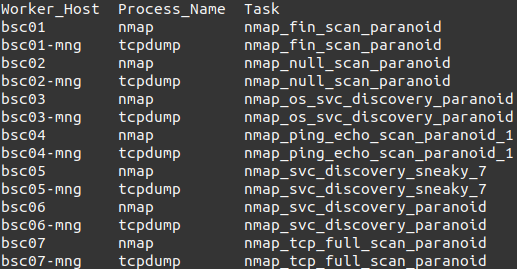
\includegraphics[scale=0.7]{images/lab/workermonitor.png}}
\caption{Capture of scan monitoring tool}
\label{fig:LabScanMonitor}
\end{figure}


Other useful tools are developed, such as the \textsc{task populator}. The populator iterates through a given task file containing tasks that want to be run a number of times in order to generate a comparable synthetic data set in the end. An incrementing number is added to the task name (e.g., $nmap\_xmas\_scan\_1$) to uniquely identify a task when iterated through by the scan deployment stage.

% retrieve.sh
A simplistic collection of captured packet captures run through a retrieve script on the scanning host, which iterates through each worker host matching a specific filter (e.g., task name) and remotely synchronizes packet captures to the local output directory on the scanning host.